\section{Теоретическая часть}

\subsection{Сведения о криптосистеме RSA}

Данный криптографический алгоритм назван в честь учёных разработавших его Rivest, Shamir и Adleman. Он основан на вычислительной сложности факторизации чисел. Алгоритм достаточно прост в освоении поэтому используется повсеместно для шифрования различных секретных сообщений и цифровых подписей. Он использует свойство односторонних функций, который обладают следующим свойством:
\begin{itemize}
	\item Если известен $x$, то $f(x)$ вычислить просто;
	\item Если известно $f(x)$, то для вычисления $x$ нет эффективного пути.
\end{itemize}

\subsection{Алгоритм создания открытого и закрытого ключа}

Криптосистема RSA генерирует ключи следующим образом:
\begin{enumerate}
	\item Выбираются два произвольных простых числа $p$ и $q$;
	\item Вычисляется модуль $n=p\cdot q$;
	\item Вычисляется значение функции Эйлера от числа $n$;
	$$
	\varphi(n)=(p-1)\cdot(q-1).
	$$
	\item Выбирается такое число $e$ в диапазоне $1 < e < \varphi(n)$, которое называется открытой экспонентой.
    Обычно выбирают простые числа из чисел Ферма: $3, 5, 17 ,256 ,65537$.
    На практике часто используется число $65537$, поскольку оно предоставляет достаточную надёжность шифрования и простоту для вычислений на ЭВМ.
    Его представление в двоичной системе счисления выглядит как $0b10000000000000001$, что объясняет лёгкость вычисления;
	\item Далее вычисляется число $d$, которое называется закрытой экспонентой и является обратным к числу $e$ по модулю $\varphi(n)$:
	$$
	d \equiv e^{-1} \Mod{\varphi(n)};
	$$
	\item В итоге пара $(e,n)$ выступает в качестве открытого ключа RSA;
	\item Пара $(d,n)$ играет роль закрытого ключа RSA.
\end{enumerate}

Однако существует множество вариаций такого подхода. Например, использование нескольких простых чисел.

\subsection{Процесс шифрования и расшифрования}

Пусть $m$ - открытый текст, который требуется зашифровать, а $c$ - шифротекст, который получится после работы алгоритма.

Шифрование выглядит следующим образом:
$$
c \equiv m^e \Mod{n};
$$

Расшифрование достаточно похожее, за исключением того, что мы используем секретную экспоненту вместо открытой:
$$
m \equiv c^d \Mod{n};
$$

Необходимое условие для работы криптосистемы RSA: $m < n$.

Корректность вычислений определяют взаимно обратные преобразования множества $\Z_n$.

Приведём простое доказательство:

Необходимо показать, что $(m^e)^d \equiv m \Mod{p \cdot q}$.

Поскольку, $e \cdot d \equiv 1 \Mod{(p-1) \cdot (q-1)} \Rightarrow ed \equiv 1 + h(p-1)(q-1)$, где $h \in \Z$.

Получим, следующую конструкцию:
\begin{align*}
    m = m^{1 + h(p-1)(q-1)} \Mod{p \cdot q} \\
    m = m \cdot m^{h(p-1)(q-1)} \Mod{p \cdot q}
\end{align*}

По малой теореме Ферма: $m^{p-1} \equiv 1 \Mod{p}$ и $m^{q-1} \equiv 1 \Mod{q}$. Следовательно,
\begin{align*}
    m^{ed} = m \cdot m^{h(p-1)(q-1)} \Mod{p \cdot q} \\
    m^{ed} = m \cdot 1^h \Mod{p \cdot q}
\end{align*}

Получим, что $m^{ed} = m \Mod{p \cdot q}. \blacksquare$


\subsection{Электронная цифровая подпись}

Электронная цифровая подпись (ЭЦП) используется для подписания сообщений различного вида для защиты от подделки документа.
Рассмотрим пример подписи документов на основе криптосистемы RSA.

Рассмотрим на примере студентов Алисы и Боба, которые являются друзьями, и преподавателя Евы.
Допустим Боб хочет получить от Алисы решение задачи для курсовой работы.
Алиса, как добрая подруга отправляет по открытым каналам связи задачу Бобу.
Однако вместо решения Бобу пришло сообщение: <<Решай свою курсовую работу сам, не списывай>>.
В итоге он обижается на Алису и перестаёт с ней дружить.

Рассмотрим более подробно. При передаче сообщения Алисой Ева перехватила её сообщение и заменила его, отправив его Бобу.
Поскольку Боб не может убедиться в том, что сообщение действительно пришло от Алисы, Ева, как преподаватель получила желаемое.
Такая атака называется MITM (Main in the middle / человек по-середине).

\begin{figure}[h!]
  \center{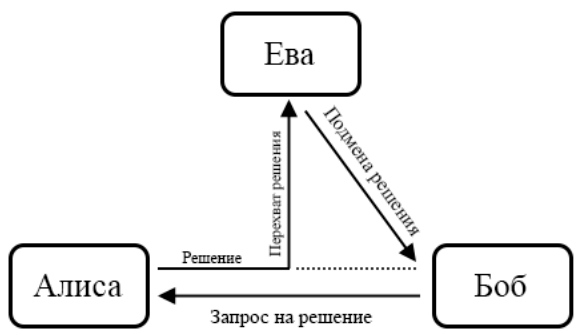
\includegraphics[scale=0.8]{img/scheme}}
  \caption{Схема атаки}
\end{figure}

Чтобы друзья остались друзьями нам нужно подтвердить личность Алисы. Для этого необходимо поменять алгоритм действий.

\begin{enumerate}
\item Боб обращается к Алисе за помощью.
\item Алиса создает пары открытого $(e_A, n_A)$ и закрытого $(d_A, n_A)$ ключей. А затем \emph{подписывает} своё решение с помощью \emph{закрытого ключа}:
\begin{align*}
    c \equiv m_A^{d_a} \Mod{n_A},\ \text{где}\  m_A - \text{решение Алисы}.
\end{align*}
\item Алиса отправляет Бобу пару свой открытый ключ $(e_A, n_A)$ и полученный шифротекст $c$.
\item Боб по открытым каналам связи получает сообщение от Алисы и проверяет корректность сообщения:
\begin{align*}
    m_A \equiv c^{e_A} \Mod{n_a}
\end{align*}
\end{enumerate}

Заметим, что даже если Ева перехватит сообщение, то она не сможет подписать исходное сообщение, поскольку у неё нет закрытого ключа $(d_A, n_A)$.

На практике же часто приходится иметь дело с большими файлами, поэтому чтобы избежать генерации большого модуля $n$ для подписи сообщения используется результат работы хэш-функций.
Например, MD5, SHA-1, SHA-256 и другич. Далее уже подписывается значение хэш-функции и отправляется вместе с сообщением.
Зачастую не требуется шифровать данные, а достаточно их подписать, для подтверждения подлинности. Рассмотрим пример как работать с хэш функциями. Обозначения ниже используются такие же, как в примерах выше за исключением $\mathrm{Hash}$ - это функция хэширования какого-то алгоритма.
\begin{table}[h!]
\centering
\begin{tabular}{c | c}
Отправитель & Получатель \\
\hline
$h = \mathrm{Hash}(m)$ & $\dot{h} = \mathrm{Hash}(M)$\\
$c \equiv h^d \Mod{n}$ & $\dot{m} \equiv c^e \Mod{n}$\\
\multicolumn{2}{c}{Осталось сравнить $\dot{m}$ и $m$}
\end{tabular}
\end{table}

В случае равенства мы можем убедиться, что документ не был модифицирован, в противном случае, документ не верный.

С помощью полученных знаний, реализуем на практике программу для создания ЭЦП на языке программирования Java.